% python figure_trans2.py --load -m fwd optim eps
\subsection{Model and Inversion of Laterally Translating Aurora}\label{sec:transverse}
The laterally translating aurora simulation was configured with $E_0\equiv \unit[5]{keV}$  and $B_{\perp,0}\in$\{1.55, 3.75\}~km. 
%
\begin{figure}
\centering
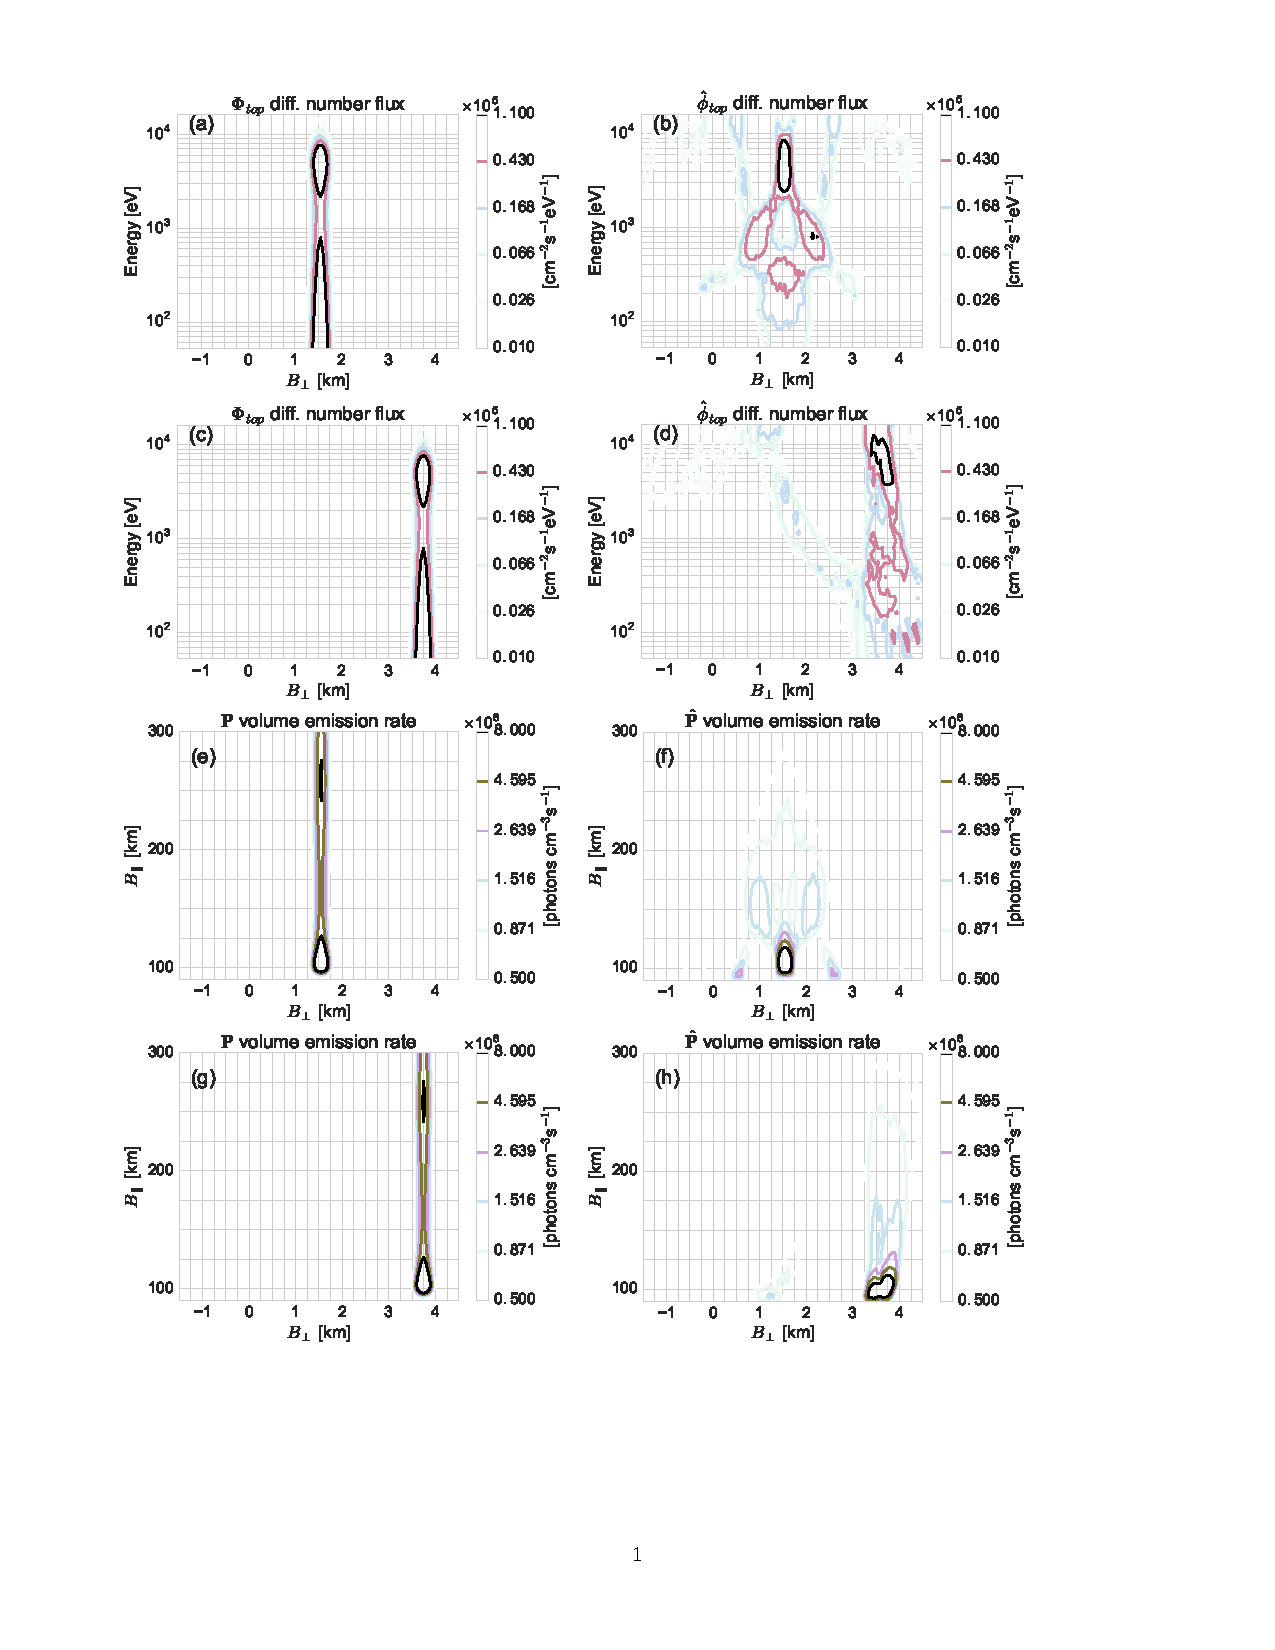
\includegraphics[trim=50 140 80 30,clip,height=0.875\textheight]{gfx/transversesim}
\caption{$B_\perp$ translating aurora simulation with characteristic energy $E_0 \equiv \unit[5]{keV}$ and $B_{\perp,0}\in$ \{1.55, 3.75\}~km. 
(a,c): differential number flux $\Phi_{top}$. (b,d): estimated differential number flux $\hat{\Phi}_{top}$. 
(e,g): forward modeled VER $\mathbf{P}$.  (f,h): estimated VER $\mathbf{\hat{P}}$.}%
\label{fig:JPB}
\end{figure}
%
Fig.~\ref{fig:JPB}(a)(c) show the input differential number flux $\Phi_{top}$, resulting in the volume emission rate $\mathbf{P}$ displayed in Fig.~\ref{fig:JPB}(e)(g). 
Fig.~\ref{fig:JPB}(b)(d) shows the estimated differential number flux $\hat{\Phi}_{top}$ using the L-BFGS-B algorithm and two cameras at $B_\perp \in\{0,3\}$ ~km.
Table~\ref{tab:Jestflame} describes the estimated differential number flux results.
The artifacts in $\hat{\Phi}_{top}$ and $\mathbf{\widehat{P}}$ come from the noise deliberately injected into the simulated $\mathbf{I}$. 
These artifacts are smaller in amplitude than the peak closest to the true answer, allowing for $\hat{\Phi}_{top,0}$ to be extracted despite the artifacts.
The estimated volume emission rate $\hat{\mathbf{P}}$ shown in Fig.~\ref{fig:JPB}(f)(h) has morphologically similar characteristics to the forward modeled volume emission rate in Fig.~\ref{fig:JPB}(e)(g), as expected. 

